%0       1         2         3         4         5         6         7         8
%2345678901234567890123456789012345678901234567890123456789012345678901234567890

\documentclass[11pt]{article}


% INCLUDE DEVELOPMENT TEXT

\newcommand{\devel}[1]{\textbf{#1}}

% EXCLUDE DEVELOPMENT TEXT

% \newcommand{\devel}[1]{}


%=======================================================================
% Document layout
%=======================================================================

\setlength{\topmargin}{0.0in}
\setlength{\oddsidemargin}{0.0in}
\setlength{\evensidemargin}{0.0in}
\setlength{\textwidth}{6.0in}
\setlength{\textheight}{9.0in}

%=======================================================================
% Packages
%=======================================================================

\usepackage{wasysym}
\usepackage{epsfig}
\usepackage{url}

%=======================================================================
% Commands
%=======================================================================

\newcommand{\cello}{\textsf{Cello}}
\newcommand{\enzo}{\textsf{Enzo}}
\newcommand{\lcaperf}{\textsf{lcaperf}}
\newcommand{\lcatest}{\textsf{lcatest}}

\newcommand{\code}[1]{\textsf{#1}}

\newcommand{\note}[1]{\devel{\eighthnote\ \textit{#1} \\}}
\newcommand{\pargraph}[1]{\devel{\P\ \textbf{#1} \\}}

\newcommand{\todo}{\devel{$\circ$}}
\newcommand{\done}{\devel{$\bullet$}}
\newcommand{\halfdone}{\devel{\textcolor{gray}{$\bullet$}}}

\newcommand{\PROJECT}{\cello}

\newcommand{\TITLE}[3]{
\title{ {\huge \PROJECT\ #1}  \\ \vspace{0.1in}
     {\small Document Version: \textbf{#3}} \vspace{-0.1in}
    }
\author{      #2 \\
        Laboratory for Computational Astrophysics\\
        University of California, San Diego}
\maketitle}

%=======================================================================


%==================================================================
% Margins and spacing
%==================================================================

\begin{document}

%=======================================================================
\TITLE{\hypre\ AMR Self-Gravity Solver}
      {James Bordner}
      {in preparation}
%=======================================================================

\tableofcontents
%======================================================================
\section{Scope}
%======================================================================

   The purpose of this document is to specify the requirements,
   describe the design and implementation, and present test results
   for \hypregrav.

%======================================================================
\section{Introduction}
%======================================================================

\hypregrav\ is a parallel self-gravity problem generator and solver.
Test problems are defined on distributed SAMR grid hierarchies, and
solved by calling the \code{SStruct} \hypre\ solver interface.

%=======================================================================
\section{Requirements} \label{s:requirements}
%=======================================================================

We break the problem into two phases: problem generation
(\code{hypre-init}), and problem solving
(\code{hypre-solve}).  

\code{hypre-init} takes as input ``high-level'' parameters
describing the problem characteristics, such as bounds on grid sizes,
number of processors, mass distribution function, etc.  The output is
a file of ``low-level'' parameters that specify the exact problem to
solve, such as grid locations, sizes, levels, and processors; point
mass locations and masses; etc.

This output file is subsequently input by \code{hypre-solve}, together
with solver-specific parameters.  A linear system is assembled and
solved using \hypre, and the solution, performance information, and
solver efficiency information, etc., are output.

%-----------------------------------------------------------------------
\subsection{\code{hypre-init}}
%-----------------------------------------------------------------------

\textbf{Input}

\begin{tabbing}
xxxxx\=xxx\=\kill\\ 
\> \todo \>  Maximum number of point masses \\
\> \todo \>  Description of probability distribution of point masses \\
\> \todo \>  Number of spheres \\
\> \todo \>  Positions of spheres \\
\> \todo \>  Masses of spheres \\
\> \todo \>  Extents of the domain \\
 \\
\> \todo \>  Lower bound on grid sizes \\
\> \todo \>  Upper bound on grid sizes \\
\> \todo \>  Upper bound on number of grids \\
 \\
\> \todo \>  AMR hierarchy depth \\
\> \todo \>  AMR Refinement factor (2,3,4) \\
\end{tabbing}

\textbf{Output}


%-----------------------------------------------------------------------
\subsection{\code{hypre-solve}}
%-----------------------------------------------------------------------

\textbf{Input}

\begin{tabbing}
xxxxx\=xxx\=\kill\\ 
\> \done \textit{dimension $<$dimension$>$} \\
\> \> \code{int dimension}
\end{tabbing}

\begin{tabbing}
xxxxx\=xxx\=\kill\\ 
\> \done \textit{sphere $<$mass$>$ $<$radius$>$ $<$center$>$} \\
\>\> \code{Scalar mass} \\
\>\> \code{Scalar radius} \\
\>\> \code{Scalar center[3]}
\end{tabbing}

\begin{tabbing}
xxxxx\=xxx\=\kill\\ 
\> \done \textit{point $<$mass$>$ $<$position$>$} \\
\>\> \code{Scalar mass} \\
\>\> \code{Scalar position[3]}
\end{tabbing}

\begin{tabbing}
xxxxx\=xxx\=\kill\\ 
\> \textit{grid} $<$id$>$ $<$parent-id$>$ $<$processor$>$ $<$low-node$>$ $<$high-node$>$ $<$node-count$>$ \\
\> \> \code{int id} $\ge 0$ \\
\> \> \code{int parent-id} $\ge 0$  \\
\> \> \code{int processor} \\
\> \> \code{Scalar vertex-lower}\code{[3]} \\
\> \> \code{Scalar vertex-upper}\code{[3]} \\
\> \> \code{int zones}\code{[3]} \textit{// Not needed? store in level if constant resolution}
\end{tabbing}

\begin{tabbing}
xxxxx\=xxx\=\kill\\ 
\> \todo \>   Type of discretization at AMR boundaries (1st-order, 2nd-order) \\
 \\
\> \todo \>    Level-0 processor distribution \\
 \\
\> \todo \>    Grid sizes \\
\> \todo \>    Grid count \\
\> \todo \>    Grid-to-processor mapping \\
 \\
\> \todo \>    Linear solver \\
\end{tabbing}

\textbf{Output}

\begin{tabbing}
xxxxx\=xxx\=\kill\\ 
\> \todo \>    Time to solution \\
\> \todo \>    Time per timestep \\
\> \todo \>    Maximum memory usage per node \\
\> \todo \>    Load balance \\
\> \todo \>    Parallel scaling \\
\end{tabbing}


%=======================================================================
\section{Design} \label{s:design}
%=======================================================================

\code{hypre-grav} reads a parameter file that defines the setup.

\begin{tabbing}
xxxxx\=xxx\=xxxxxxxx\=\kill\\ 
\> \todo \> \code{int}  \>   \code{dimension}     \\
\\
\> \todo \> \code{float} \>  \code{particle\_position\_clumpiness}  \\
\> \todo \> \code{float} \>  \code{particle\_mass\_clumpiness} \\
\> \todo \> \code{float} \>  \code{particle\_mass\_average} \\
\\
\> \todo \> \code{float} \>  \code{sphere\_center[3]} \\
\> \todo \> \code{float} \>  \code{sphere\_radius} \\
\> \todo \> \code{float} \>  \code{sphere\_mass} \\
\\
\> \todo \> \code{float} \>  \code{domain\_extents[3]} \\
\\
\> \todo \> \code{int} \>    \code{processor\_count[3]} \\
\\
\> \todo \> \code{string} \>  \code{discretization\_type \{"linear", "quadratic"\}} \\
\\
\> \todo \> \code{int} \>    \code{grid\_count[3]} \\
\> \todo \> \code{int} \>    \code{grid\_size[3]} \\
\\
\> \todo \> \code{int} \>    \code{amr\_depth} \\
\> \todo \> \code{int} \>    \code{amr\_grid\_count[N]} \\
\> \todo \> \code{int} \>    \code{amr\_grid\_size[N]} \\
\> \todo \> \code{string} \>    \code{amr\_load\_balance \{"none", "size"\}} \\
\\
\> \todo \> \code{string} \>  \code{solver \{"cg","fac"\}}
\end{tabbing}

Outputs

\begin{enumerate}
\item Time to solution
\item Time per timestep
\item Maximum memory usage per node
\item Load balance
\item Parallel scaling
\end{enumerate}

%-----------------------------------------------------------------------
\subsection{Classes} \label{ss:classes}
%-----------------------------------------------------------------------

%-----------------------------------------------------------------------
\subsubsection{\code{Problem} class}


\begin{tabbing}
xxxx\=xxxxxxxxxxxxxxxxxxx\=xxxxxxxxx\=\kill\\ 
\>  \code{int} \> \code{dimension}                     \> \textit{Problem dimenion} \\
\>  \code{std::vector$<$Sphere *$>$} \> \code{spheres} \> \textit{List of sphere masses} \\
\>  \code{std::vector$<$Sphere *$>$} \> \code{points}  \> \textit{List of point masses} \\
\>  \code{std::vector$<$Grid *$>$} \> \code{grids}   \> \textit{List of grids defining the hierarchy} \\
\end{tabbing}

%-----------------------------------------------------------------------
\subsubsection{\code{Sphere} class}

\begin{tabbing}
xxxx\=xxxxxxxxxxxxxxxxxxx\=xxxxxxxxx\=\kill\\ 
\>  \code{static int} \> \code{d\_}    \> \textit{Dimension} \\
\>  \code{Scalar *} \> \code{x\_}   \> \textit{Position} \\
\>  \code{Scalar} \> \code{r\_}    \> \textit{Radius} \\
\>  \code{Scalar} \> \code{m\_}    \> \textit{Mass} \\
\end{tabbing}

%-----------------------------------------------------------------------
\subsubsection{\code{Grid} class}

\begin{tabbing}
xxxx\=xxxxxxxxxxxxxxxxxxx\=xxxxxxxxx\=\kill\\ 
\>  \code{static int} \> \code{d\_}   \> \textit{Spacial dimension} \\
\>  \code{int} \> \code{p\_}   \> \textit{Processor rank} \\
\>  \code{int} \> \code{l\_}   \> \textit{Hierarchy level (root==0)} \\
\>  \code{Scalar *} \> \code{xl\_}  \> \textit{Lower position} \\
\>  \code{Scalar *} \> \code{xu\_}  \> \textit{Upper position} \\
\>  \code{int *} \> \code{n\_}   \> \textit{Number of zones (excluding ghosts)} \\
\end{tabbing}

%=======================================================================
\subsection{Discretization} \label{s:discretization}
%=======================================================================

\newcommand{\indvar}{r}
 \newcommand{\uc}{u(\indvar)}

 \newcommand{\uxp}{u(\indvar+h_x)}
 \newcommand{\uxm}{u(\indvar-h_x)}
 \newcommand{\uxph}{u(\indvar+\frac{h_x}{2})}
 \newcommand{\uxmh}{u(\indvar-\frac{h_x}{2})}

 \newcommand{\uyp}{u(\indvar+h_y)}
 \newcommand{\uym}{u(\indvar-h_y)}
 \newcommand{\uyph}{u(\indvar+\frac{h_y}{2})}
 \newcommand{\uymh}{u(\indvar-\frac{h_y}{2})}

 \newcommand{\uzp}{u(\indvar+h_z)}
 \newcommand{\uzm}{u(\indvar-h_z)}
 \newcommand{\uzph}{u(\indvar+\frac{h_z}{2})}
 \newcommand{\uzmh}{u(\indvar-\frac{h_z}{2})}

 \newcommand{\ac}{a(\indvar)}
 \newcommand{\axph}{a(\indvar+\frac{h_x}{2})}
 \newcommand{\axmh}{a(\indvar-\frac{h_x}{2})}
 \newcommand{\ayph}{a(\indvar+\frac{h_y}{2})}
 \newcommand{\aymh}{a(\indvar-\frac{h_y}{2})}
 \newcommand{\azph}{a(\indvar+\frac{h_z}{2})}
 \newcommand{\azmh}{a(\indvar-\frac{h_z}{2})}

 \newcommand{\alc}{\alpha^{000}}
 \newcommand{\alxp}{\alpha^{100}}
 \newcommand{\alxm}{\alpha^{\bar{1}00}}
 \newcommand{\alyp}{\alpha^{010}}
 \newcommand{\alym}{\alpha^{0\bar{1}0}}
 \newcommand{\alzp}{\alpha^{001}}
 \newcommand{\alzm}{\alpha^{00\bar{1}}}

 \newcommand{\Uc}{U^{000}}
 \newcommand{\Uxp}{U^{100}}
 \newcommand{\Uxm}{U^{\bar{1}00}}
 \newcommand{\Uyp}{U^{010}}
 \newcommand{\Uym}{U^{0\bar{1}0}}
 \newcommand{\Uzp}{U^{001}}
 \newcommand{\Uzm}{U^{00\bar{1}}}

\begin{center}
\begin{minipage}{1.5in}
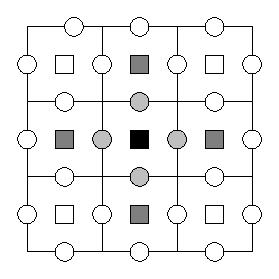
\epsfig{file=fig/stencil.eps,width=1.5in}
\end{minipage} \[ \nabla\cdot(\ac \nabla \uc) = \bar{\rho} \]
\end{center}


 \begin{eqnarray*}
 \nabla\cdot(\ac \nabla \uc) & = & D_x (\ac D_x \uc) + D_y (\ac D_y \uc) + D_z (\ac D_z \uc) \\
 & \approx & \frac{\delta_{h_x}}{h_x} (\ac \frac{\delta_{h_x}}{h_x} \uc) + 
             \frac{\delta_{h_y}}{h_y} (\ac \frac{\delta_{h_y}}{h_y} \uc) + 
             \frac{\delta_{h_z}}{h_z} (\ac \frac{\delta_{h_z}}{h_z} \uc) \\
 & \approx & \frac{1}{h_x^2}\delta_{h_x} (\ac \delta_{h_x} \uc) + 
             \frac{1}{h_y^2}\delta_{h_y} (\ac \delta_{h_y} \uc) + 
             \frac{1}{h_z^2}\delta_{h_z} (\ac \delta_{h_z} \uc) \\
 & = & \frac{1}{h_x^2}\delta_{h_x} (\ac (\uxph - \uxmh))\\
 & + & \frac{1}{h_y^2}\delta_{h_y} (\ac (\uyph - \uymh)) \\
 & + & \frac{1}{h_z^2}\delta_{h_z} (\ac (\uzph - \uzmh)) \\
 & = & \frac{1}{h_x^2} (\axph (\uxp - \uc)) - (\axmh (\uc - \uxm)) \\
 & + & \frac{1}{h_y^2} (\ayph (\uyp - \uc)) - (\aymh (\uc - \uym)) \\
 & + & \frac{1}{h_z^2} (\azph (\uzp - \uc)) - (\azmh (\uc - \uzm)) \\
 & = & \frac{1}{h_z^2} \azmh \uzm + \frac{1}{h_y^2} \aymh \uym + \frac{1}{h_x^2} \axmh \uxm \\
 & - & [\frac{1}{h_x^2} \axph  + \frac{1}{h_x^2} \axmh \\
 & &+  \frac{1}{h_y^2} \ayph  + \frac{1}{h_y^2} \aymh \\
 & & +  \frac{1}{h_z^2} \azph  + \frac{1}{h_z^2} \azmh] \uc \\
 & + &  \frac{1}{h_x^2} \axph \uxp + \frac{1}{h_y^2} \ayph \uyp  + \frac{1}{h_z^2} \azph \uzp \\
 & = & \alzm\Uzm +  \alym\Uym +  \alxm\Uxm \\
 & + & \alc\Uc \\
 & + & \alxp\Uxp +  \alyp\Uyp +  \alzp\Uzp 
 \end{eqnarray*}

 \begin{eqnarray}
 \alzm & \equiv & \frac{1}{h_z^2} \azmh \\
 \alym & \equiv & \frac{1}{h_y^2} \aymh \\
 \alxm & \equiv & \frac{1}{h_x^2} \axmh \\
 \alc  & \equiv & - [\frac{1}{h_x^2} \axph  + \frac{1}{h_x^2} \axmh \\
 & + & \frac{1}{h_y^2} \ayph  + \frac{1}{h_y^2} \aymh \\
 & + & \frac{1}{h_z^2} \azph  + \frac{1}{h_z^2} \azmh] \\
 \alxp & \equiv & \frac{1}{h_x^2} \axph \\
 \alyp & \equiv & \frac{1}{h_y^2} \ayph \\
 \alzp & \equiv & \frac{1}{h_z^2} \azph \\
 \end{eqnarray}

\begin{center}
\begin{minipage}{1.5in}
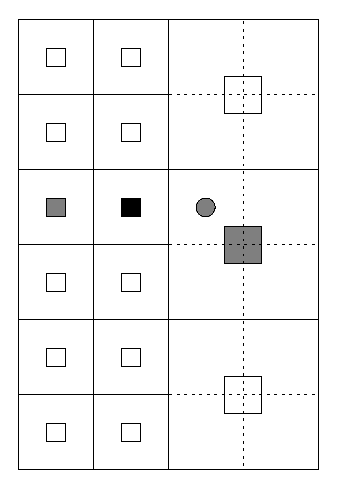
\epsfig{file=fig/stencil0.eps,width=1.5in}
\end{minipage}
\end{center}
\begin{center}
\begin{minipage}{1.5in}
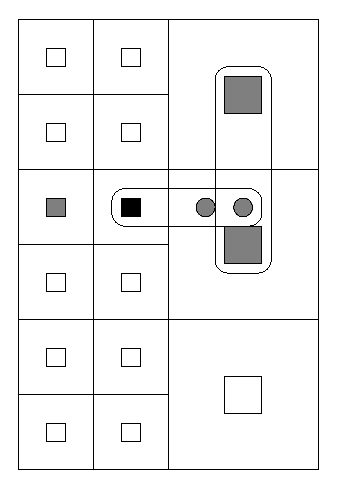
\epsfig{file=fig/stencil1.eps,width=1.5in}
\end{minipage}
\end{center}
\begin{center}
\begin{minipage}{1.5in}
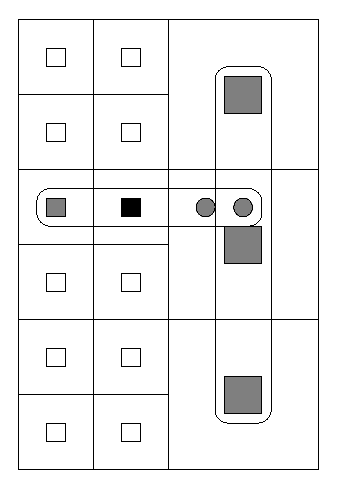
\epsfig{file=fig/stencil2.eps,width=1.5in}
\end{minipage}
\end{center}



\begin{center}
\begin{minipage}{2in}
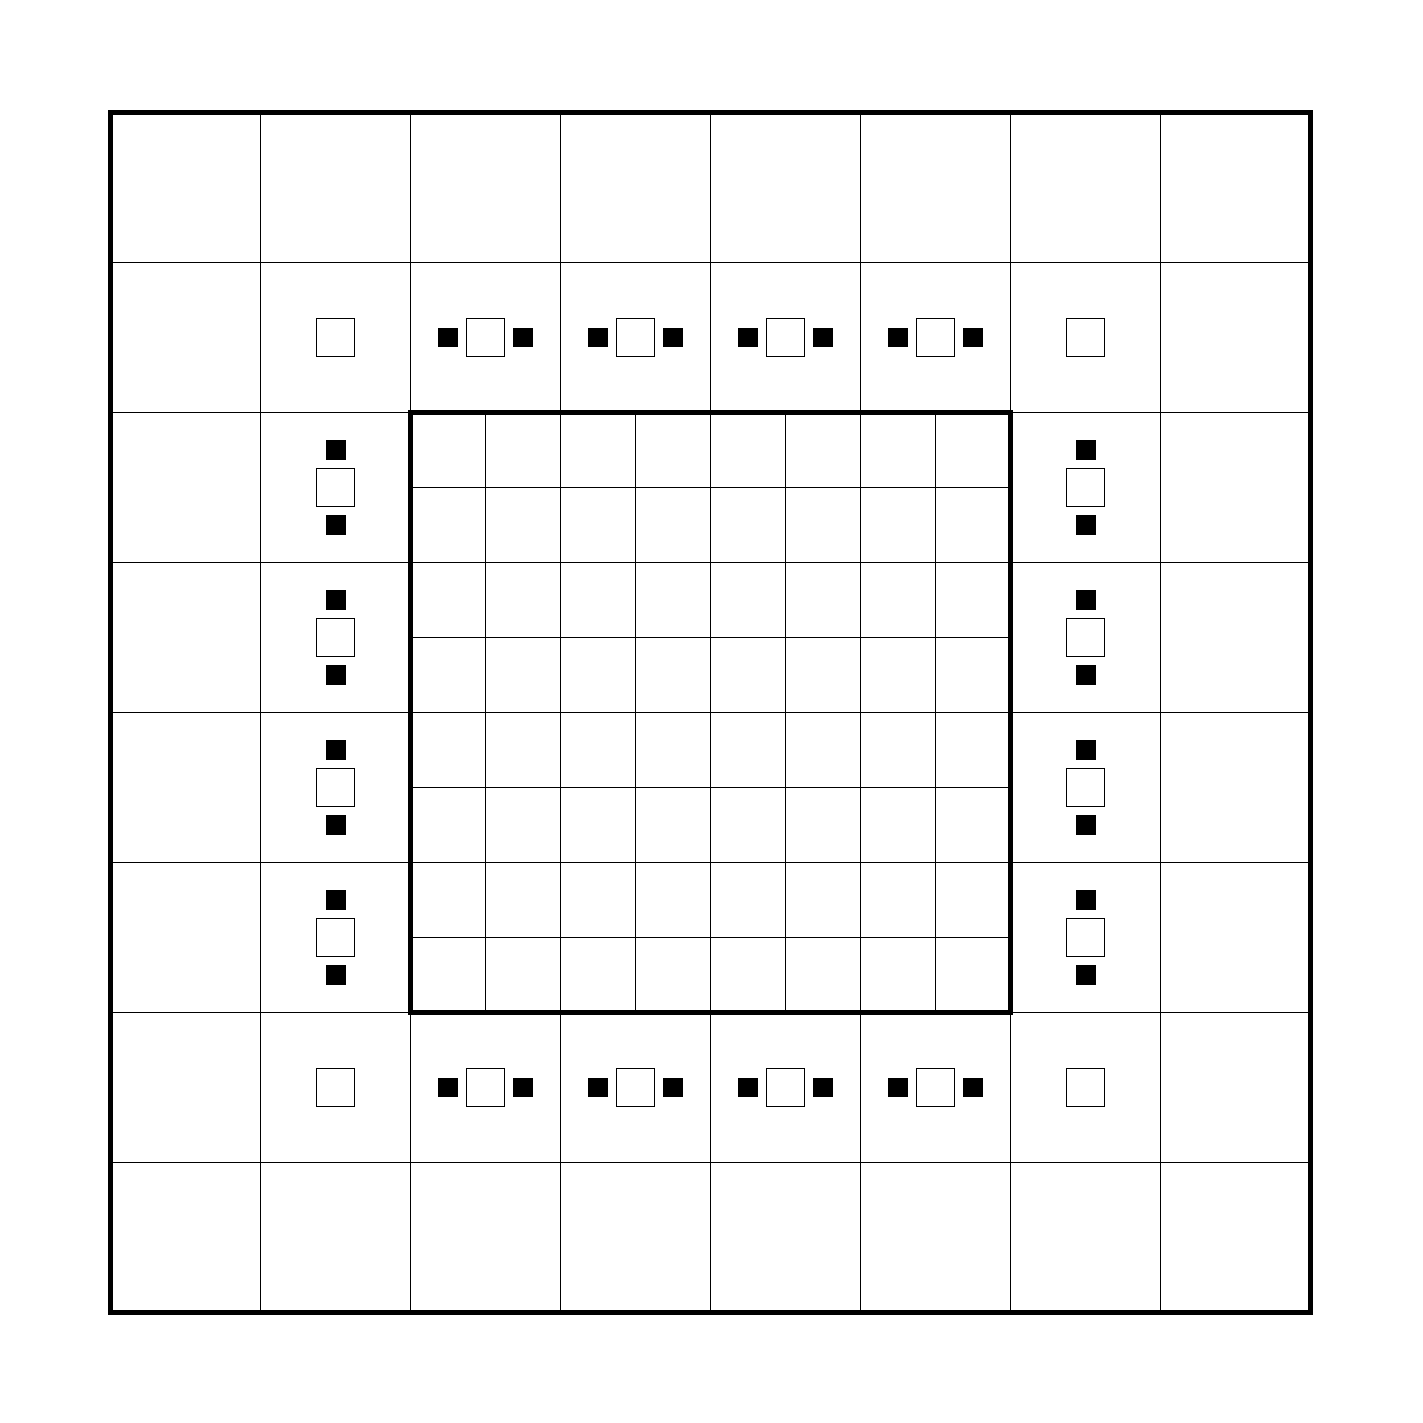
\epsfig{file=fig/discret6.eps,width=2.0in}
\end{minipage}$\Rightarrow$
\begin{minipage}{2in}
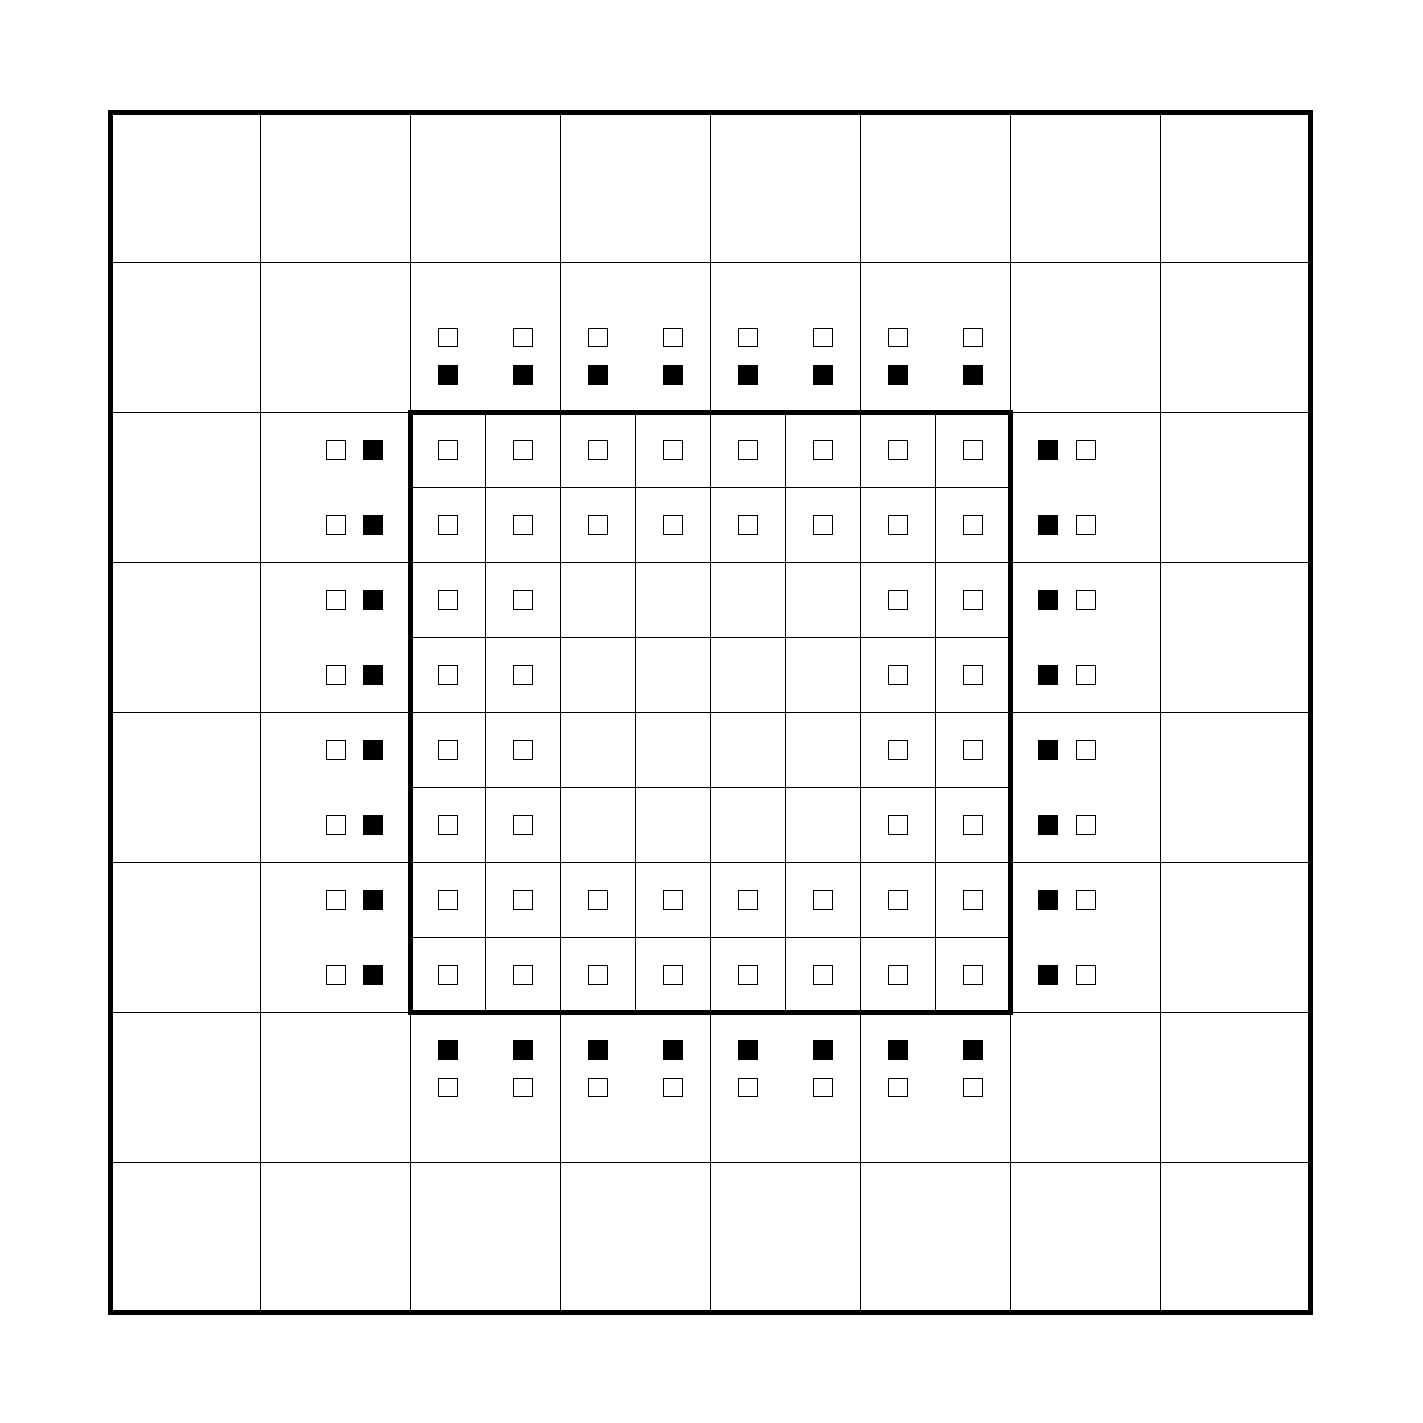
\epsfig{file=fig/discret5.eps,width=2.0in}
\end{minipage}$\Rightarrow$
\begin{minipage}{2in}
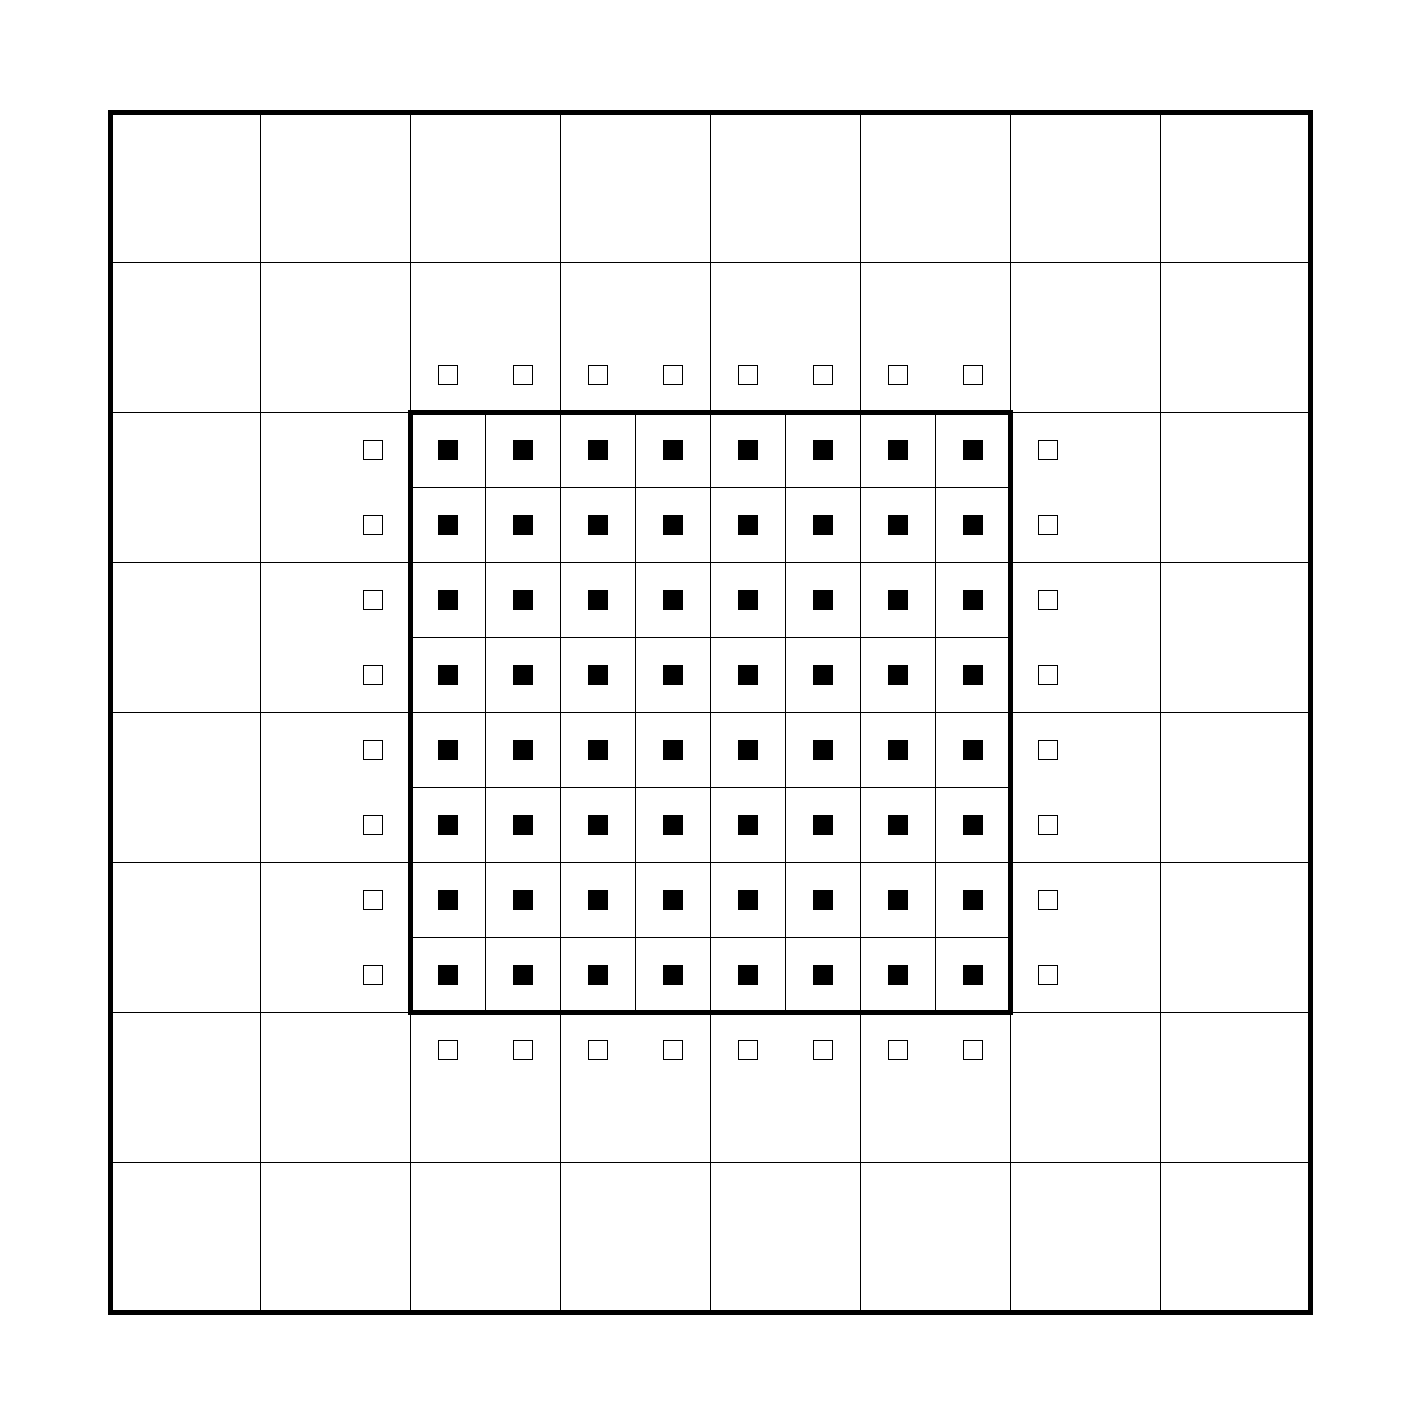
\epsfig{file=fig/discret4.eps,width=2.0in}
\end{minipage} \\
\begin{minipage}{4.5in}
\hfill $\Downarrow$
\end{minipage} \\
\begin{minipage}{2in}
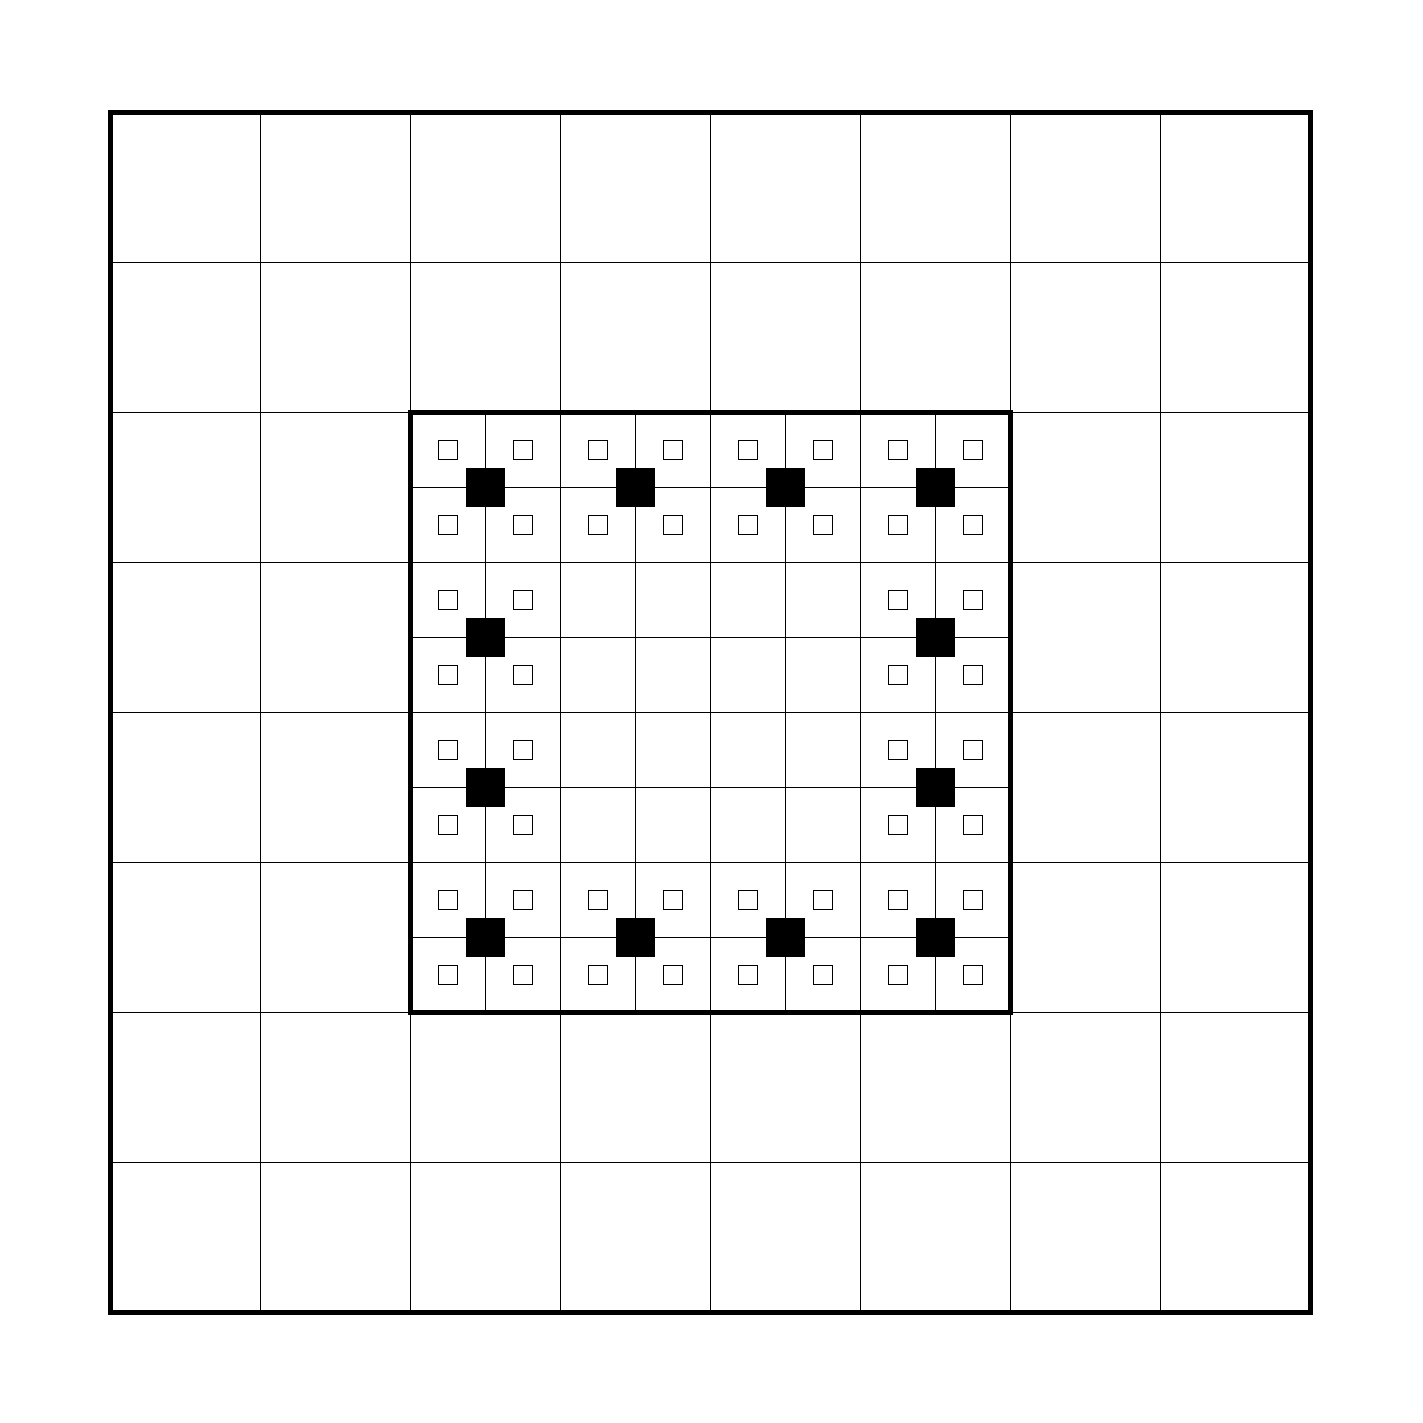
\epsfig{file=fig/discret3.eps,width=2.0in}
\end{minipage}$\Rightarrow$
\begin{minipage}{2in}
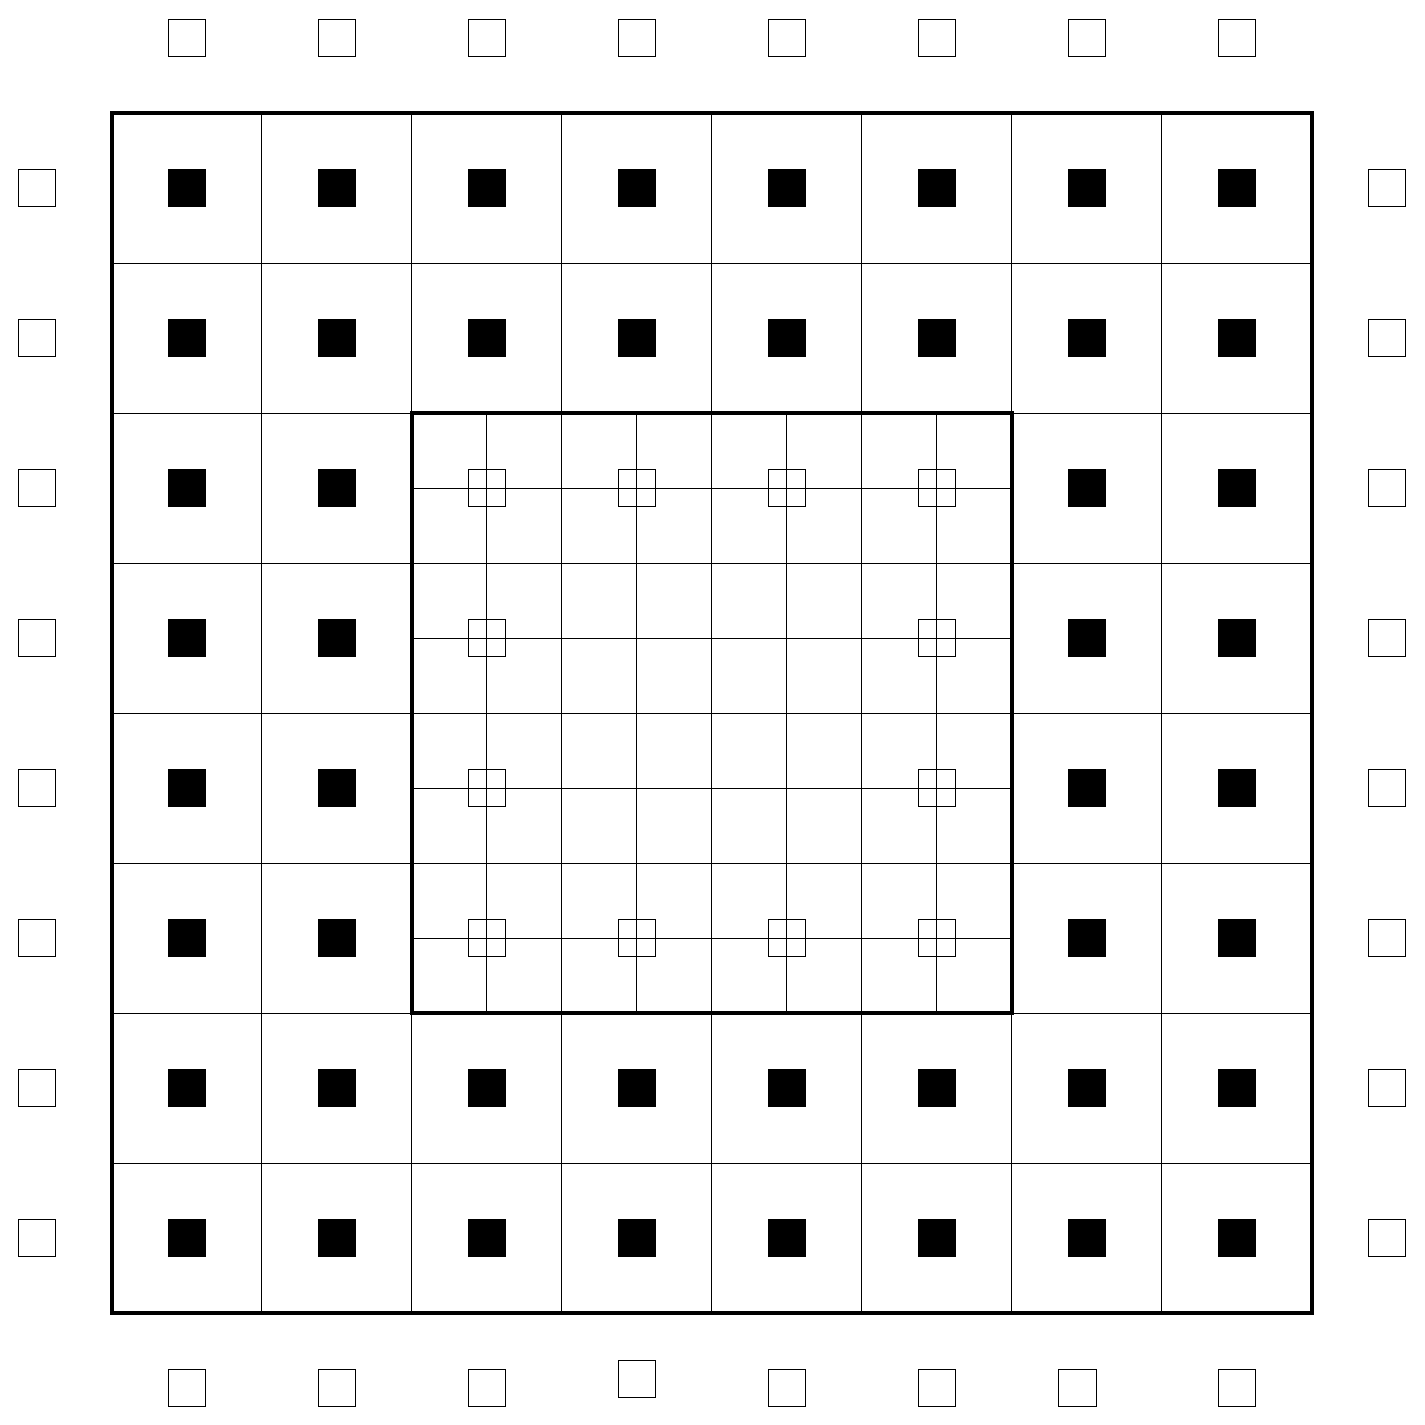
\epsfig{file=fig/discret2.eps,width=2.0in}
\end{minipage}$\Rightarrow$
\begin{minipage}{2in}
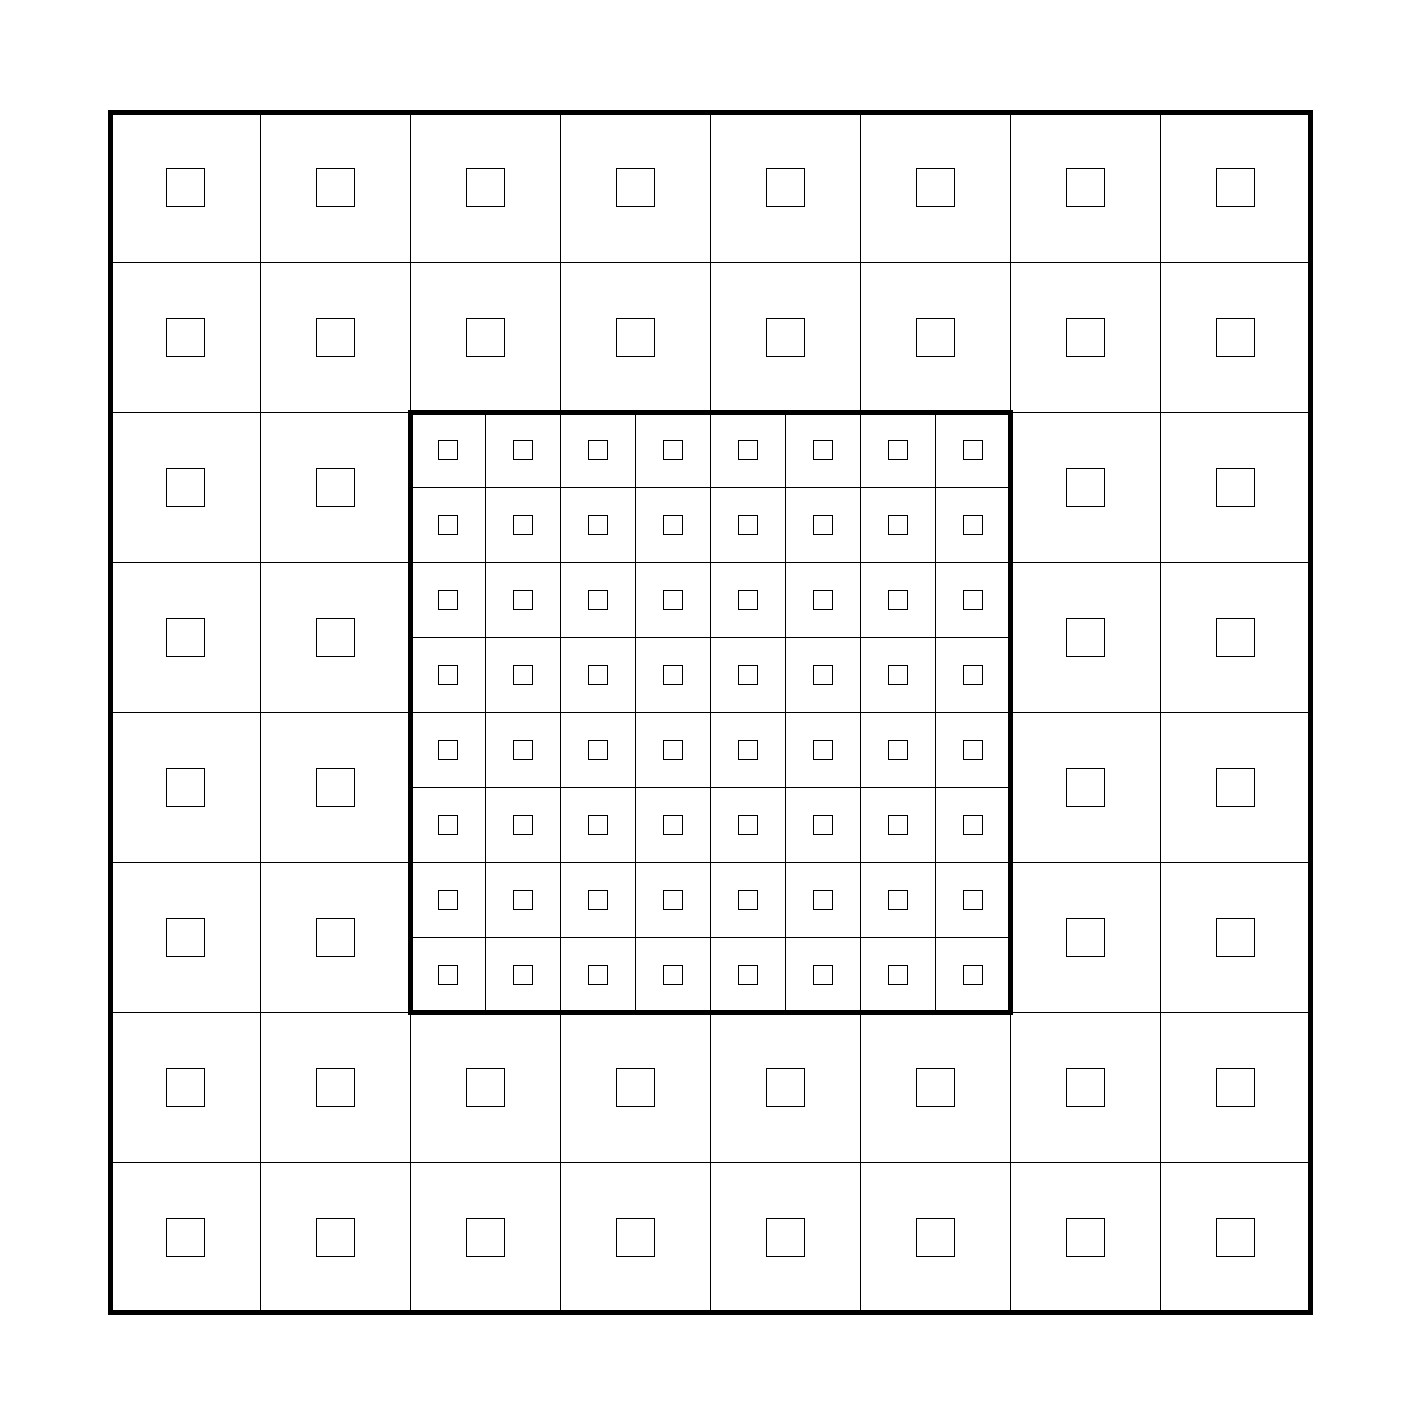
\epsfig{file=fig/discret1.eps,width=2.0in}
\end{minipage}
\end{center}

\begin{center}
\begin{minipage}{6.0in}
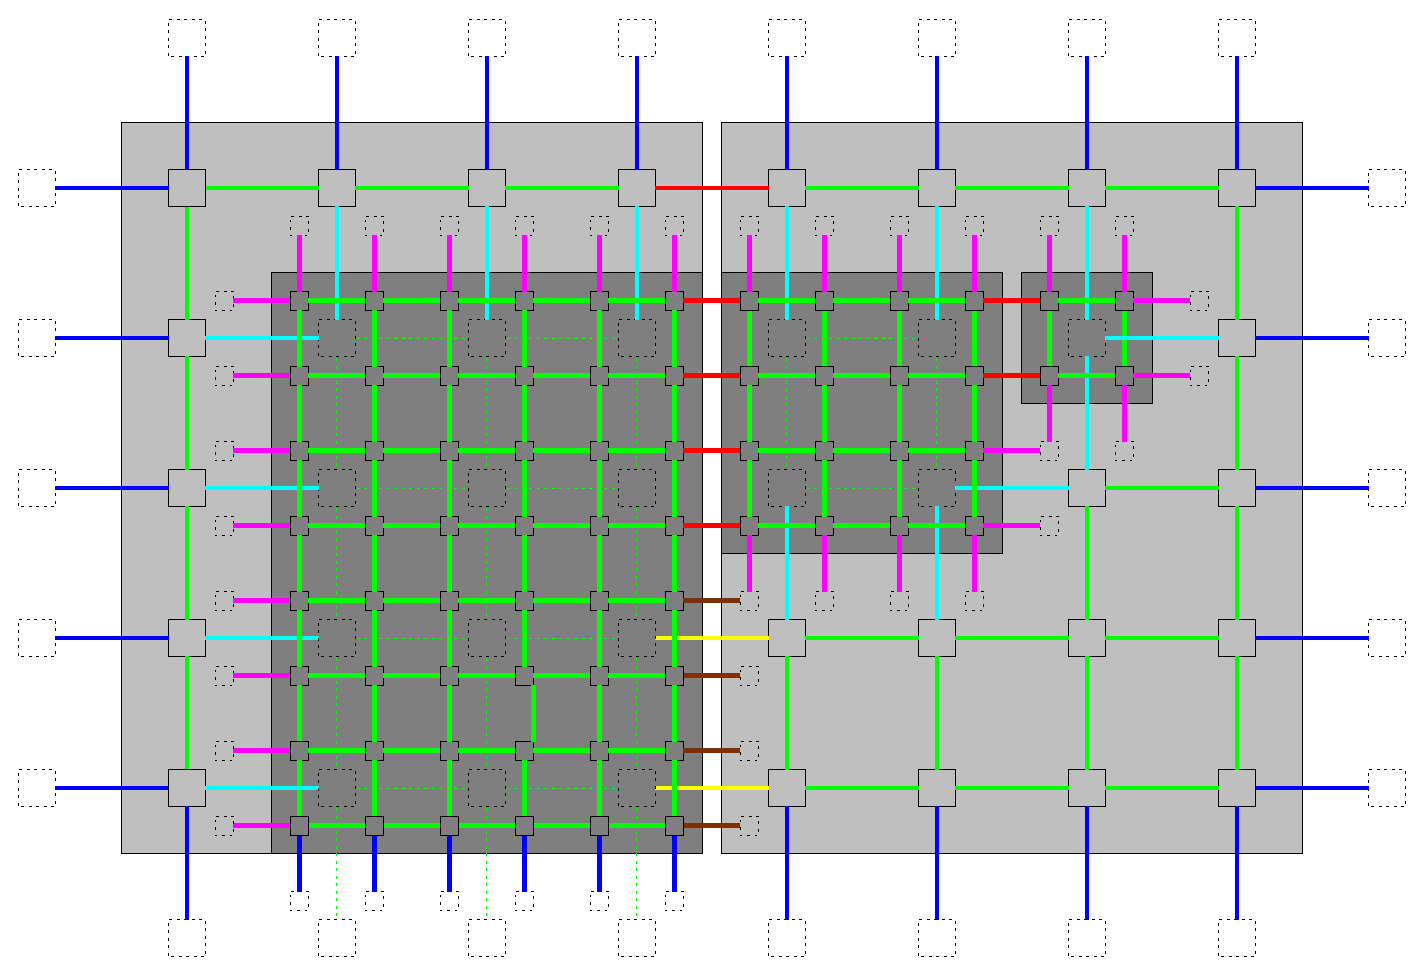
\epsfig{file=fig/discret-step-1.eps,width=6.0in}
\end{minipage}
\end{center}

Grid patches are controlled using
\begin{itemize}
\item \code{HYPRE\_SStructGridCreate()}
\item \code{HYPRE\_SStructGridSetExtents()}
\item \code{HYPRE\_SStructGridSetVariables()}
\item \code{HYPRE\_SStructGridSetNeighborBox()}
\item \code{HYPRE\_SStructGridAssemble()}
\item \code{HYPRE\_SStructGridSetNumGhost()}
\item \code{HYPRE\_SStructGridDestroy()}
\end{itemize}

Stencils are controlled using
\begin{itemize}
\item \code{HYPRE\_SStructStencilCreate()}
\item \code{HYPRE\_SStructStencilSetEntry()}
\item \code{HYPRE\_SStructStencilDestroy()}
\end{itemize}

Graphs are controlled using
\begin{itemize}
\item \code{HYPRE\_SStructGraphCreate()}
\item \code{HYPRE\_SStructGraphSetStencil()}
\item \code{HYPRE\_SStructGraphAddEntry()}
\item \code{HYPRE\_SStructGraphSetObjectType()}
\item \code{HYPRE\_SStructGraphAssemble()}
\item \code{HYPRE\_SStructGraphDestroy()}
\end{itemize}

Matrices are controlled using
\begin{itemize}
\item \code{HYPRE\_SStructMatrixCreate()}
\item \code{HYPRE\_SStructMatrixInitialize()}
\item \code{HYPRE\_SStructMatrixGetObject()}
\item \code{HYPRE\_SStructMatrixSetObjectType()}
\item \code{HYPRE\_SStructMatrixSetValues()}
\item \code{HYPRE\_SStructMatrixAddToValues()}
\item \code{HYPRE\_SStructMatrixSetBoxValues()}
\item \code{HYPRE\_SStructMatrixAddToBoxValues()}
\item \code{HYPRE\_SStructMatrixDestroy()}
\item \code{HYPRE\_SStructMatrixPrint()}
\end{itemize}

Vectors are controlled using:
\begin{itemize}
\item \code{HYPRE\_SStructVectorCreate()}
\item \code{HYPRE\_SStructVectorInitialize()}
\item \code{HYPRE\_SStructVectorGetObject()}
\item \code{HYPRE\_SStructVectorSetObjectType()}
\item \code{HYPRE\_SStructVectorSetValues()}
\item \code{HYPRE\_SStructVectorAddToValues()}
\item \code{HYPRE\_SStructVectorSetBoxValues()}
\item \code{HYPRE\_SStructVectorAddToBoxValues()}
\item \code{HYPRE\_SStructVectorDestroy()}
\item \code{HYPRE\_SStructVectorPrint()}
\end{itemize}




Types of matrix elements for a given unknown:

\begin{tabular}{ll}
\textcolor{green}{internal} & \code{HYPRE\_SStructStencilSetEntry()} \\
\textcolor{green}{overlapped internal} & \code{HYPRE\_SStructStencil} \\
\textcolor{red}{neighbor} & \code{HYPRE\_SStructGridSetNeighborBox()}\\
\textcolor{blue}{boundary} & \code{HYPRE\_SStructGraphAddEntries()}\\
\textcolor{magenta}{fine-coarse parent} & \code{HYPRE\_SStructGraphAddEntries()}\\
\textcolor{cyan}{coarse-fine child} & \code{HYPRE\_SStructGraphAddEntries()}\\
\textcolor{brown}{fine-coarse parent--neighbor} & \code{HYPRE\_SStructGraphAddEntries()}\\
\textcolor{yellow}{coarse-fine neighbor--child} & \code{HYPRE\_SStructGraphAddEntries()}\\
\end{tabular}

%=======================================================================
\section{Testing} \label{s:testing}
%=======================================================================

\EndDOCUMENT

\end{document}
%==================================================================

